\chapter{Risk Analysis}

\section{Introduction}
This section describes the several possible risks associated with the project. The first subsection contains descriptions of the different columns in the Risk Analysis table. The second subsection contains the table itself, which lists details such as the numerous risks and their associated levels of severity and consequences. 

\section{Table Description}
Name of Risk: Specifically identifies specific risks associated with project.\newline
Consequences: The outcome of the risks if they occur.\newline
Probability: The likelihood of the risk occurring.\newline
Severity: The effect the risk can impose on the project.\newline
Impact: The probability multiplied by the severity. It determines a quantitative measurement of the risk on the project.\newline
Mitigation Strategies: Possible actions to take to prevent the risks from occurring.\newline

\begin{figure}[!ht]
	\centering
    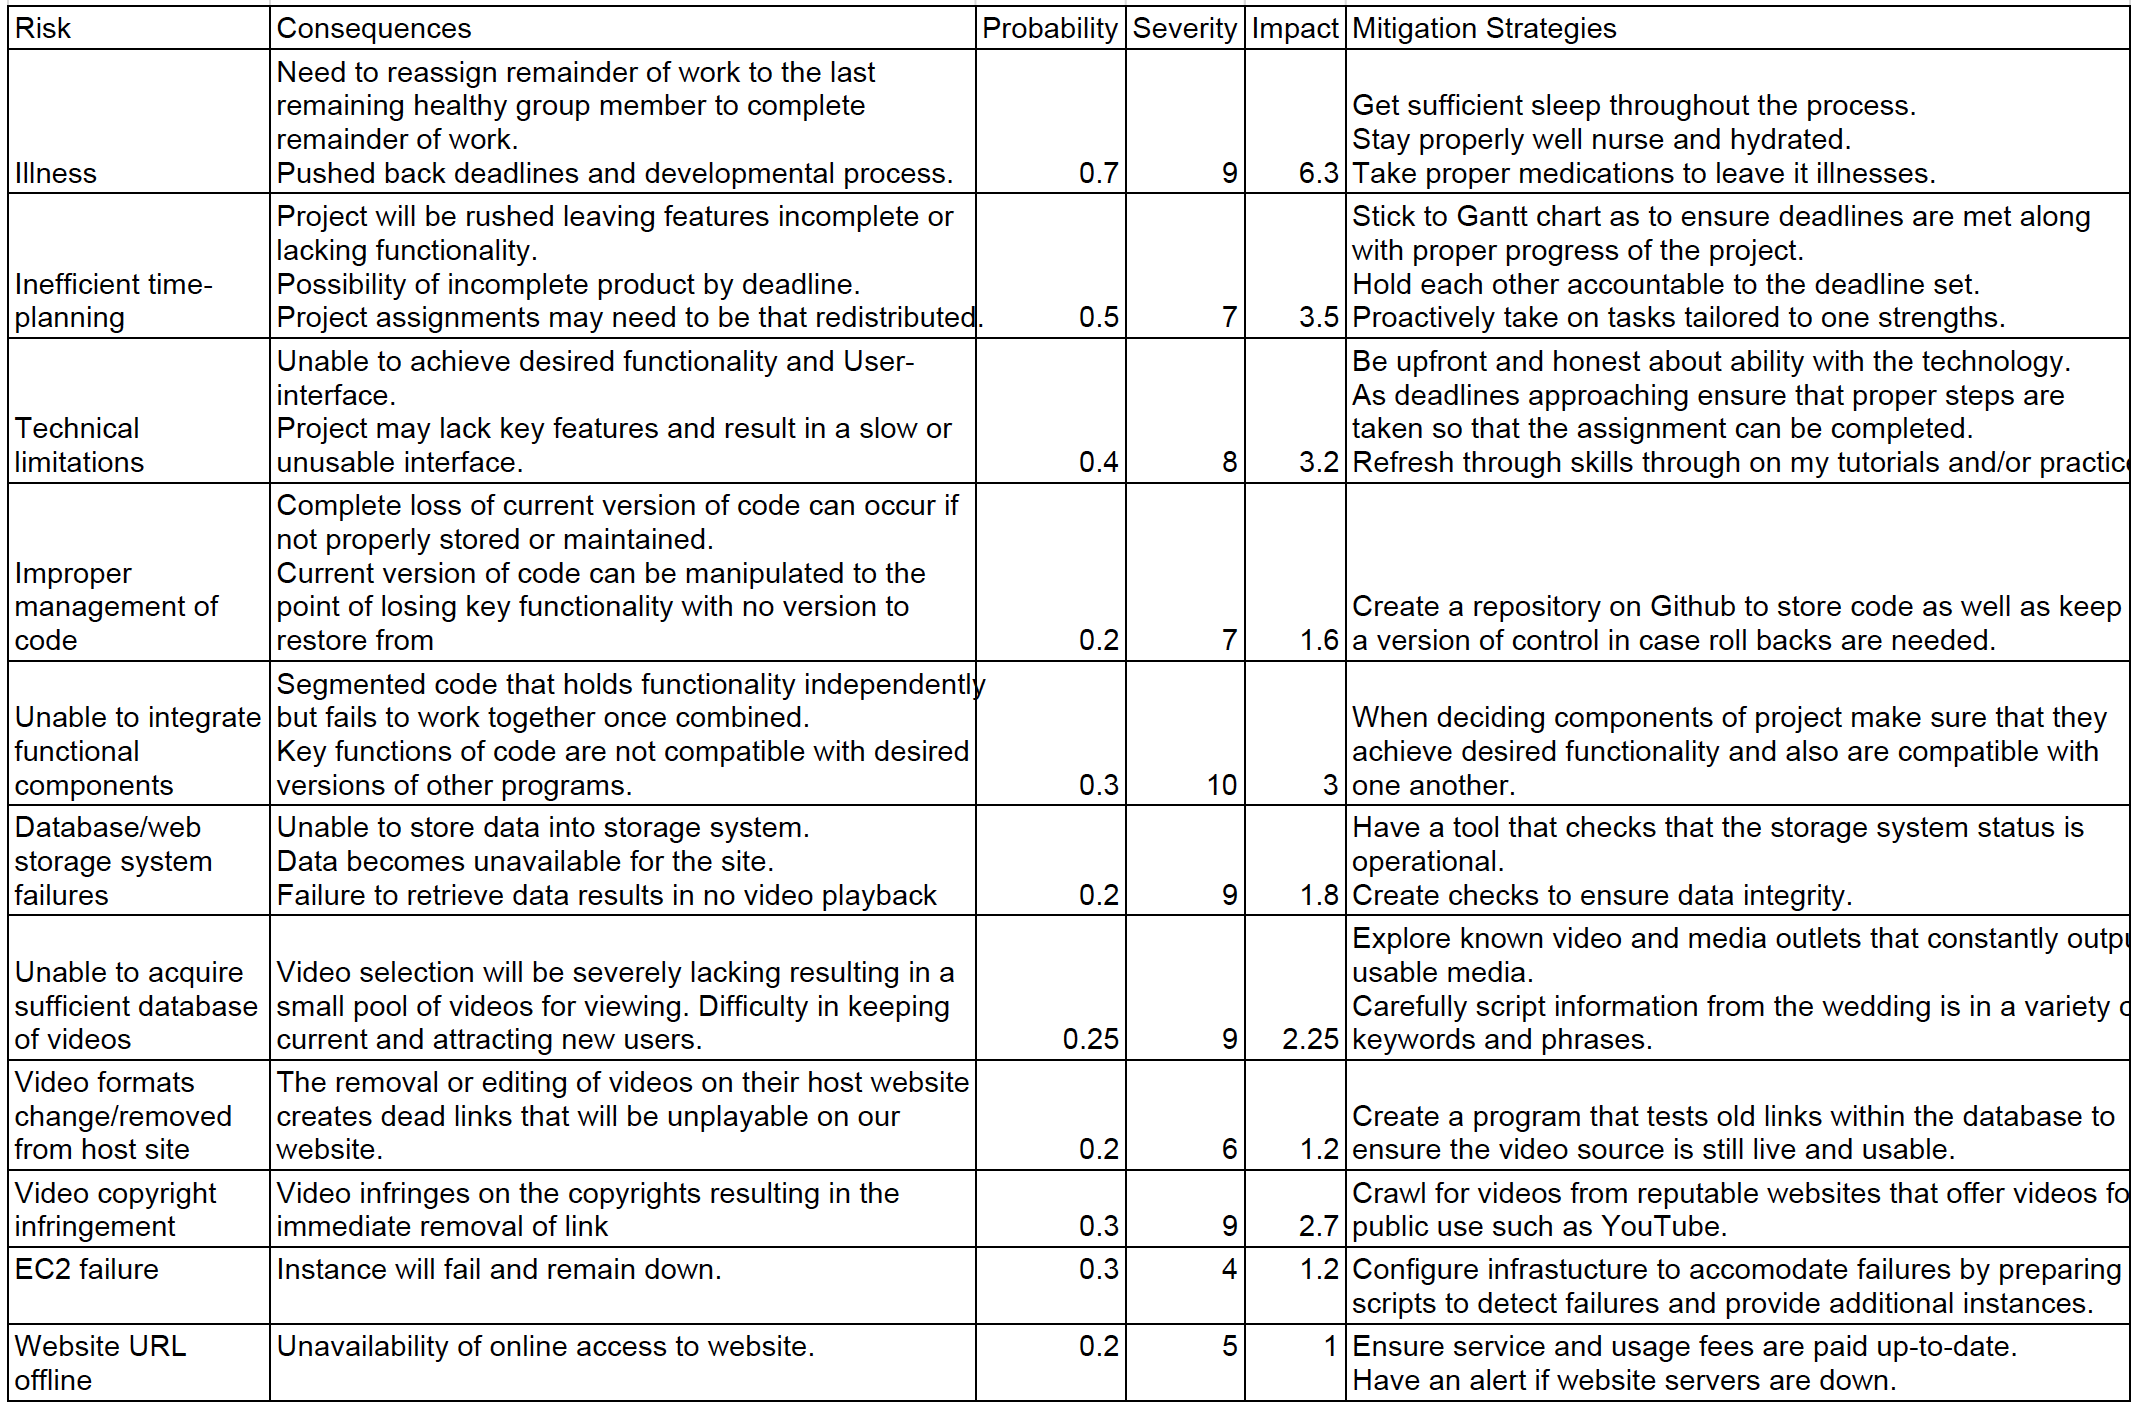
\includegraphics[width=\textwidth]{riskTable}
    \caption{Risk Analysis Table}
\end{figure}